\chapter{The Researchers Perspective}
\label{researchers_perspective}
	\section{Introduction}
		In this section, we will briefly look at the available features for the researcher of the project. 
		Every scientist working in prediction models for thyroid nodule classification may upload its algorithm 
		on the platform and receive helpful feedback about its performance using the Researcher panel explained below. 
		Visually the researcher's panel is nearly identical to the administrator panel explained in chapter 
		\ref{admin_perspective} but offers access to the different data than the administrator panel. This is done 
		to reduce costs and reuse the similar functionality developed for the administrator panel. The researcher panel 
		is provided by the Predictor Service(Task Backend).
		\begin{figure}[H]
			\iftrue
			\caption{Predictor Service}
			\centering
			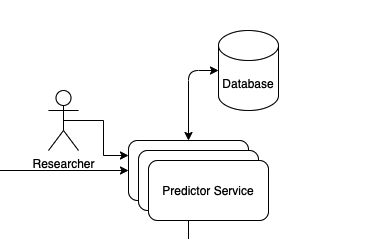
\includegraphics[scale=0.5]{figures/taskbe}
			\fi
		\end{figure}
	\section{Researcher Panel}
		The researcher panel provides an interface to the researcher to view its algorithm outputs and performance in an easy and user-friendly manner.
		\begin{note}
			To connect to the researcher panel, we need to connect to the following addresses\\
			\begin{center}
				(if online) https://uortmc-taskbe.herokuapp.com/admin/ \\
				(local machine )http://127.0.0.1:3002/admin
			\end{center}
			Please refer to chapter \ref{start-stop-guide} for more details around how to connect.
		\end{note}
		\subsection{Login screen}
			\begin{figure}[H]
				\iftrue
				\caption{Researcher panel login screen}
				\centering
				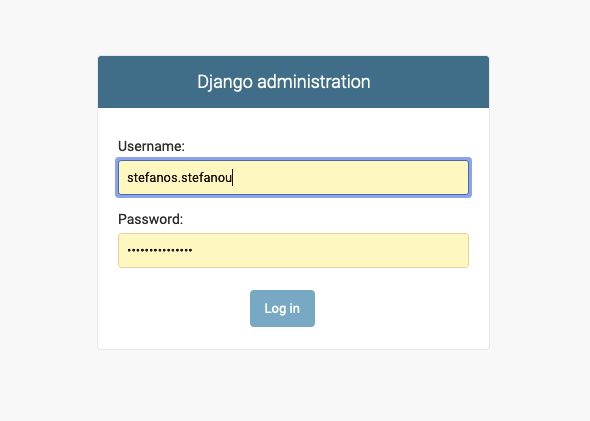
\includegraphics[scale=0.5]{figures/research-panel-login}
				\fi
			\end{figure}
			The login screen is the first screen that an researcher should encounter. The information transmitted into the Predictor
			Service is encrypted using HHTPS[\cite{rfc2818}] and transformed to an salted[\cite{MANBER1996171}] MD5 Hash[\cite{rfc1321}] 
			for maximum possible security. 
		\subsection{Researcher Panel Features}
			\begin{figure}[H]
				\iftrue
				\caption{Researcher Panel-Home}
				\centering
				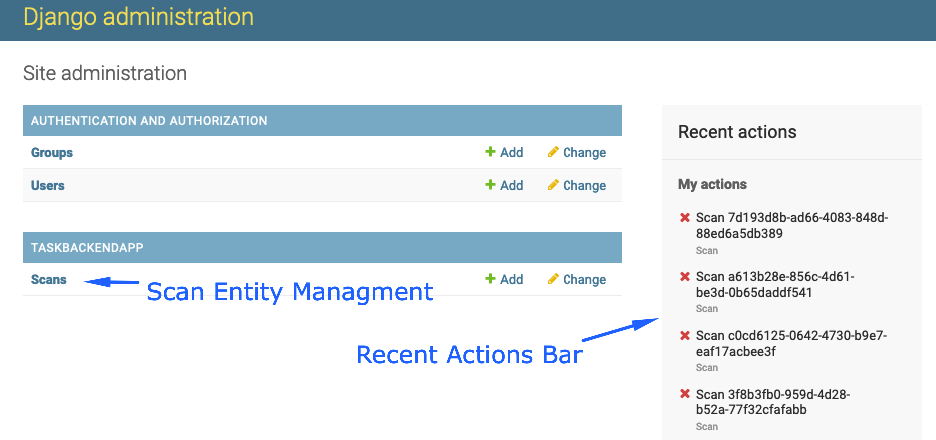
\includegraphics[scale=0.3]{figures/research-panel-home}
				\fi
			\end{figure}
			After the login sequence is completed, the researcher will be redirected to the panel's home page; there, 
			it has available all the functionality needed to perform debbuging into the algorithm under develepoment, such as 
			real-time logging capability. By selecting the scan in question can have access to the required information
			\begin{figure}[H]
				\iftrue
				\caption{Researcher Panel-List of scans}
				\centering
				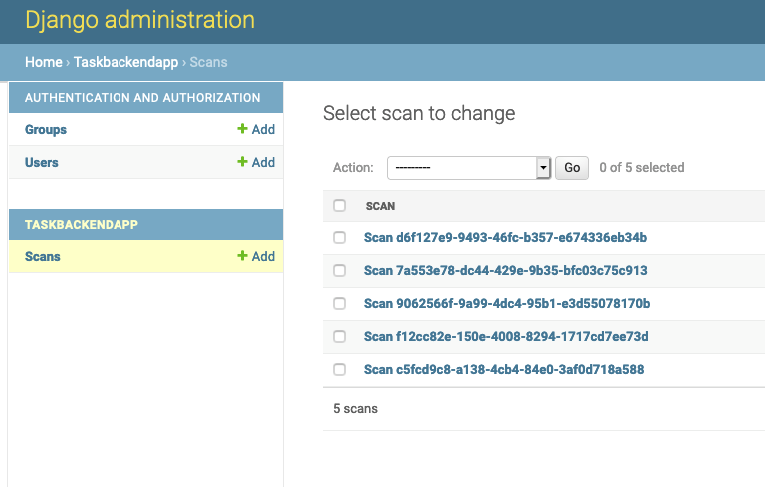
\includegraphics[scale=0.3]{figures/research-panel-scan-list}
				\fi
			\end{figure}
			\begin{figure}[H]
				\iftrue
				\caption{Researcher Panel-Scan Details Example}
				\centering
				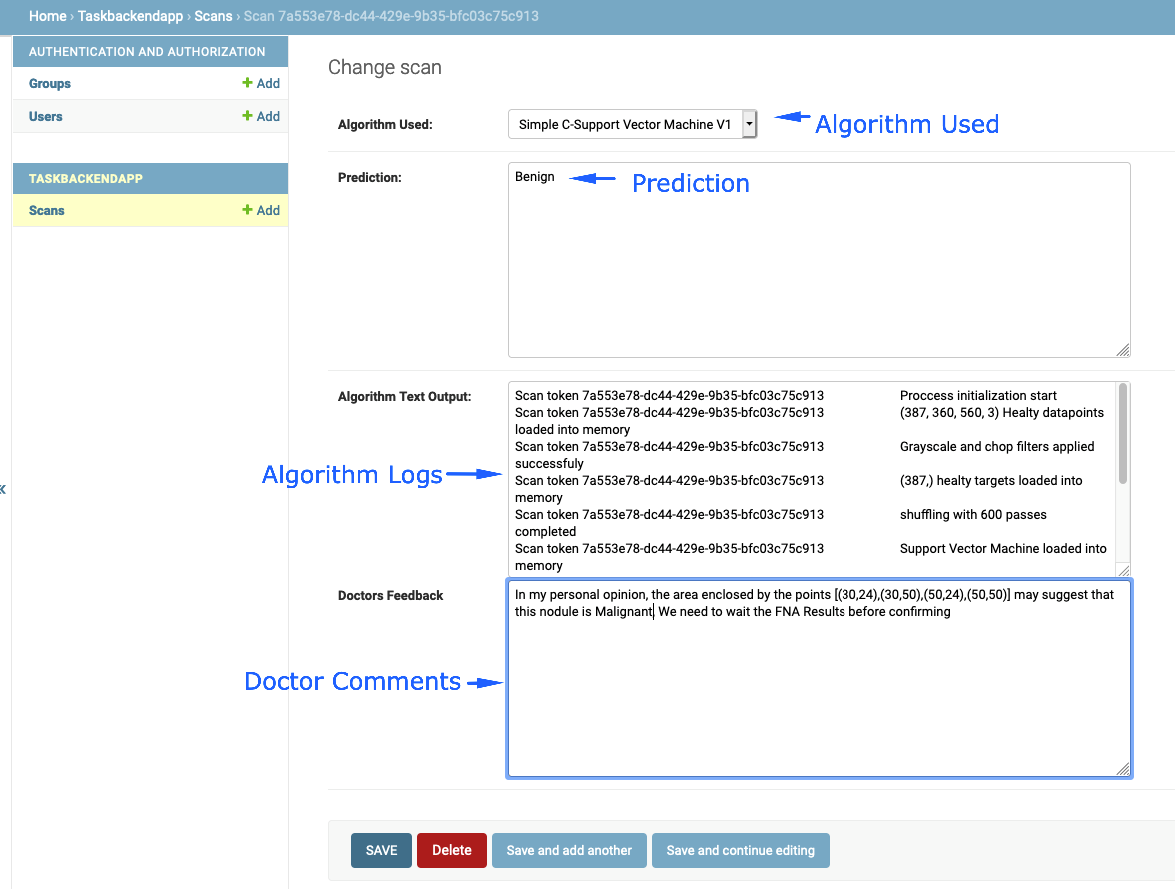
\includegraphics[scale=0.3]{figures/research-panel-scan-view}
				\fi
			\end{figure}
			The researcher then can improve the algorithm based on the feedback provided from the doctors, as well as to troubleshoot
			possible errors using the real-time logging capability.
			
			
			
			
		
		
		
			
			
			
			
			
		
	



